\documentclass{article}
\usepackage[margin=1in]{geometry} % Adjust the page margins
% For better handling of math expressions
\usepackage{amsmath}

% For better formatting of lists
\usepackage{enumitem}

% Optional for improved typography
\usepackage{microtype}
\usepackage[margin=1in]{geometry} % Adjust margins as needed
\usepackage{lipsum} % Provides sample text. Remove this for your actual document.
\usepackage[table,xcdraw]{xcolor}
\usepackage{colortbl}
\usepackage{graphicx} % Required for including images
\usepackage{graphicx}
\usepackage{textcomp}
\usepackage{xcolor}
\usepackage{float}
\usepackage{amsmath}
\usepackage{longtable}
\usepackage{booktabs}
\usepackage{multicol}
\usepackage{multirow}
\usepackage[margin=0.7in]{geometry}

\usepackage{algorithm} % For algorithms
\usepackage{algpseudocode} % For pseudocode

\usepackage{pdflscape} % For landscape orientation
\usepackage{xltabular} % Extended tabular with auto page break and X columns
\usepackage{booktabs} % For better table formatting
\usepackage[table]{xcolor} % For cell coloring
\usepackage{makecell} % For line breaks within cells
\usepackage{listings} % For including code-like listings
\usepackage{xcolor} % For color definitions in listings

\lstset{
    basicstyle=\ttfamily\small,
    columns=fullflexible,
    frame=single,
    breaklines=true,
    postbreak=\mbox{\textcolor{red}{$\hookrightarrow$}\space},
    keywordstyle=\color{blue},
    numbers=left,
    stepnumber=1,
}
% Define a new centered column type with adjustable width
\newcolumntype{C}[1]{>{\centering\arraybackslash}p{#1}}

\title{Robustness of DL Models (Local and Global Properties)}
\author{Arooj Arif}
\date{\today} % You can also specify a date manually

\begin{document}

\maketitle % This command creates the title
\section{Overview}

\subsection{Problem Statement}
In the past few years, deep neural networks (DNNs) have made remarkable progress in achieving human-level performance. With the broader deployment of DNNs on various safety critical systems like autonomous, healthcare, avionics, etc., the concerns over their safety and trustworthiness have been raised in public, particularly highlighted by incidents involving self-driving cars.

An important low-level requirement for DNNs is that they are robustness against input perturbations. DNNs have been shown to suffer from a lack of robustness because of their susceptibility to adversarial examples such that small modifications to an input, sometimes imperceptible to humans, can make the network unstable.

\subsection{Robustness Category}
\begin{itemize}
    \item \textbf{Offensive} 
       \begin{itemize} % Start of nested itemize
        \item focus on heuristic approach to find adversarial examples that are close as possible to correct input
    \end{itemize} % End of nested itemize
     \item \textbf{Defensive}
            \begin{itemize} % Start of nested itemize
        \item focus on increase the robustness of DNNs (test and verify system to provide robustness guarentee)
    \end{itemize} % End of nested itemize
\end{itemize} 

\subsection{Limitations of DNNs}
   \begin{itemize}
     \item existing mechanisms depend on manual collections of labelled data that cause \textbf{unguided simulation}
     \item input space is extremely large, \textbf{unguided simulation} are higly unlikely to find erroneous behavior
    \end{itemize}

\subsection{DNN Safety and Trustworthy (4 Aspects)}

\begin{itemize}

    \item \textbf{Testing} 
    \begin{itemize} % Start of nested itemize
        \item \textbf{Coverage Criteria}
         \item \textbf{Test Case Generation}
    \end{itemize} % End of nested itemize

    \item Verification
     \item Adversarila attacks and Defences
    \item Interpretability

\end{itemize}

\subsection{Problems in DNN Testing}
DNNs testing techniques aim to discover bugs, through finding counter examples that challenge the system's correctness, or to establish confidence by rigorously evaluating the system with numerous test cases. These testing techniques are computationally less expensive and therefore are able to work with state-of-the- art DNNs. However, DL testing has some limitations:
\begin{itemize}
    \item Standards available in industry but \textbf{Lack of Logcial Structure} and \textbf{System Specification}  
     \item Heavily depend on manual collections of test data under different conditions which become expensive as number of test condition increases
\end{itemize}

\subsection{Research Goal}

   \begin{itemize}
     \item Evaluate local and global robustness of DNNs
    \end{itemize}
    
\subsection{Research Quesitons}
\begin{itemize}
 \item How to specify relevant local robustness properties?
 \item How to explore input-output space efficiently?
 \item How to generate realistic input to automate such exploration?
 \item How to automatically collect test data that detect erroneous behavior?
 \item How to design comprehensive framework?
\end{itemize}
  




\begin{landscape}
\begin{xltabular}{\linewidth}{|>{\raggedright\arraybackslash}X|>{\raggedright\arraybackslash}X|>{\raggedright\arraybackslash}p{3.5cm}|>{\raggedright\arraybackslash}p{6cm}|>{\raggedright\arraybackslash}p{2.5cm}|>{\raggedright\arraybackslash}p{3cm}|} % Adjust '3cm' as needed
\caption{Summary of Test Methodologies and Their Characteristics} \\
\hline
\rowcolor[HTML]{EFEFEF} 
\textbf{Methodology} & \textbf{Dataset} & \textbf{Benchmark} & \textbf{Limitation/Future Work} & \textbf{Coverage Criteria} & \textbf{Test Generation} \\ \endhead

Symbolic execution with local explainability. LIME provides explanations for predictions\cite{Agarwal} & German Credit Data, Adult census income, Bank marketing, US Executions, Fraud Detection, Raw Car Rentals, Credit data, Census data & THEMIS (Algorithm) The technique produces 3.72 times more successful test cases than existing state-of-the-art. & FW: Expand to text and image domains FW: Measure symbolic execution efficacy using neuron coverage, boundary value coverage. & -- & Symbolic/Concolic \\ \hline


Concolic testing method \cite{Youcheng} & \makecell[lt]{- MNIST\\ - CIFAR-10} & DeepXplore, DeepTest, DeepCover, and DeepGauge & & \makecell[lt]{NC, SSC, NBC} & Concolic \\ \hline
\cellcolor[HTML]{FFFFFF}Whitebox framework for testing DL systems, introducing neuron coverage for test measurement \cite{Kexin}& \makecell[lt]{- MNIST\\ - ImageNet\\ - Driving\\ - VirusTotal\\ - Drebin} & \makecell[lt]{LeNet variations\\ State-of-the-art\\ image classifiers \\ Nvidia DAVE \\ PDF malware detectors\\ Android app\\ malware detectors} & Inherits differential testing constraints. & NC & Dual-optimisation \\ \hline
Automates testing for DNN-driven autonomous cars \cite{Yuchi}& Udacity self driving car challenge 2 & \makecell[lt]{Chauffeur-\\ Epoch\\ Rambo-S1\\ Rambo-S2\\ Rambo-S3} & \makecell[lt]{L:missing some realistic cases.\\ L: restricted only steering angle,\\ not focus on brake and accelerator\\ L: cannot simulate complex road scene}. & NC & Greedy search \\ \hline
White box methodology, Proposed four novel test criteria tailored to DNN, structural features. able to capture and quantify causal relations existing in a DNN, Achieved balance between bug finding ability and computational cost \cite{Sun}  & MNIST, CIFAR-10, ImageNet & State-of-the-art neural networks of different sizes (from a few hundred up to millions of neurons) to demonstrate their utility with respect to four aspects: bug finding, DNN safety statistics, testing efficiency, DNN internal structure analysis & & MC/DC & Symbolic execution \\ \hline
Proposed criteria facilitate the understanding of DNNs as well as the test data quality from different levels and angles\cite{Ma} & \makecell[lt]{MNIST, ImageNet} & \makecell[lt]{LeNet-1\\ LeNet-4\\ LeNet-5,\\ VGG-19,\\ ResNet-50} & \makecell[lt]{More diverse datasets \\and DL architectures needed.\\ Check on real-world systems.} & NBC & Gradient descent methods \\ \hline
An unsupervised learning framework to synthesize realistic driving scenes to test inconsistent behaviors\cite{Zhang} & Udacity Training Udacity Test Ep1 Udacity Test Ep2 Youtube Ep1 Youtube Ep2 & Autumn, Chauffeur & \makecell[lt]{Lack a good standard to evaluate image\\ quality (i.e., realism). Udacity dataset is \\relatively small and the \\autonomous driving models are \\quite simple. Only focus on steering\\ wheel.} & -- & Mutation testing \\ \hline
An automated fuzz testing framework for hunting potential defects of general-purpose DNNs\cite{Xie} & MNIST, CIFAR-10, ImageNet & \makecell[lt]{LeNet-1\\ LeNet-4\\ LeNet-5\\ RN-20\\ VGG-16\\ MobileNet\\ RN-50} & NC cannot generate effective results to evaluate the models with various quality. NC is less effective in error triggering test detection and sensitive defect detection. & \makecell[lt]{NC\\ KMNC\\ NBC\\ SNAC\\ KNC\\ KNC} & Metamorphic mutation \\ \hline

\end{xltabular}

\end{landscape}



\section{Experiments} 
\subsection{Pipeline to generate adversarial Example} 
\begin{itemize}
    \item \textbf{Dataset}: MNIST , CIFAR
    \item \textbf{Model}:CNN, Andriushchenko2020Understanding', 'Carmon2019Unlabeled', 'Sehwag2020Hydra', 'Wang2020Improving', 'Hendrycks2019Using'

    \item \textbf{Library} Foolbox
\end{itemize}
\begin{lstlisting}[language=Python, caption=Python code for generating attack examples]
# Function to perform an attack, plot results, and return attack data
def perform_attack(attack, attack_name):
    
    raw_advs, clipped_advs, success = attack(fmodel, images, labels, epsilons=epsilons)

    for i, (eps, advs_) in enumerate(zip(epsilons, clipped_advs)):
        y_adv = np.argmax(model.predict(advs_), axis=1)

    attack_results = {
        'raw_advs': raw_advs,
        'clipped_advs': clipped_advs,
        'success': success
    }

    return attack_results

# Convert data to TensorFlow tensors
images = tf.convert_to_tensor(correct_examples)
labels = tf.convert_to_tensor(correct_labels, dtype=tf.int32)

# Create a Foolbox model for TensorFlow
fmodel = fb.TensorFlowModel(model, bounds=(0, 1))

# Define epsilons
epsilons = [0.01, 0.02, 0.03, 0.04, 0.05, 0.1, 0.2, 0.3, 0.4, 0.5]

# Perform AdditiveUniformNoise attack
additive_results = perform_attack(fb.attacks.LinfAdditiveUniformNoiseAttack(), "AdditiveUniformNoise")

# Perform PGD attack
pgd_results = perform_attack(fb.attacks.LinfPGD(), "PGD")

# Perform FastGradientAttack attack
guassian_results = perform_attack(fb.attacks.LinfFastGradientAttack(), "FastGradientAttack")
\end{lstlisting}


\begin{table}[htbp]
\centering
\caption{Summary of Robust Accuracy for Different Perturbations}
\label{tab:robust_accuracy}
\begin{tabular}{lcccccccccc} % Corrected: Now 11 columns are defined
\toprule
\textbf{Perturbation} & \textbf{0.01} & \textbf{0.02} & \textbf{0.03} & \textbf{0.04} & \textbf{0.05} & \textbf{0.1} & \textbf{0.2} & \textbf{0.3} & \textbf{0.4} & \textbf{0.5} \\
\midrule
PGD                  & 99.2\% & 97.9\% & 95.4\% & 91.2\% & 84.8\% & 22.4\% & 0.0\%  & 0.0\%  & 0.0\%  & 0.0\% \\
Additive             & 100.0\% & 99.9\% & 99.9\% & 99.8\% & 99.8\% & 99.5\% & 98.7\% & 95.5\% & 88.9\% & 77.2\% \\
FastGradient         & 99.4\% & 98.6\% & 97.1\% & 95.5\% & 92.9\% & 69.5\% & 17.9\% & 2.4\%  & 0.4\%  & 0.3\% \\
\bottomrule
\end{tabular}
\end{table}

\begin{longtable}{cccccc}
\caption{Adversarial Attack Robustness Across Models and Epsilon Values} \\
\toprule
\textbf{Epsilon} & \textbf{Model} & \textbf{Attack} & \textbf{Robust Acc} & \textbf{Time (ms)} \\
\midrule
\endfirsthead

\multicolumn{5}{c}%
{\tablename\ \thetable\ -- \textit{Continued from previous page}} \\
\toprule
\textbf{Epsilon} & \textbf{Model} & \textbf{Attack} & \textbf{Robust Acc} & \textbf{Time (ms)} \\
\midrule
\endhead

\bottomrule
\multicolumn{5}{r}{\textit{Continued on next page}} \\
\endfoot

\bottomrule
\endlastfoot
0.01 & Andriushchenko2020Understanding & FGSM & 0.74 & 16 \\
0.01 & Andriushchenko2020Understanding & PGD & 0.736 & 13334 \\
0.01 & Andriushchenko2020Understanding & DeepFool & 0.72 & 16982 \\
0.01 & Andriushchenko2020Understanding & BIM & 0.736 & 2807 \\
0.01 & Carmon2019Unlabeled & FGSM & 0.844 & 2965 \\
0.01 & Carmon2019Unlabeled & PGD & 0.838 & 112636 \\
0.01 & Carmon2019Unlabeled & DeepFool & 0.834 & 109733 \\
0.01 & Carmon2019Unlabeled & BIM & 0.838 & 24465 \\
0.01 & Sehwag2020Hydra & FGSM & 0.852 & 18 \\
0.01 & Sehwag2020Hydra & PGD & 0.848 & 110397 \\
0.01 & Sehwag2020Hydra & DeepFool & 0.846 & 133199 \\
0.01 & Sehwag2020Hydra & BIM & 0.848 & 23801 \\
0.01 & Wang2020Improving & FGSM & 0.83 & 17 \\
0.01 & Wang2020Improving & PGD & 0.83 & 112763 \\
0.01 & Wang2020Improving & DeepFool & 0.816 & 189376 \\
0.01 & Wang2020Improving & BIM & 0.83 & 24344 \\
0.01 & Hendrycks2019Using & FGSM & 0.824 & 17 \\
0.01 & Hendrycks2019Using & PGD & 0.822 & 111587 \\
0.01 & Hendrycks2019Using & DeepFool & 0.82 & 161093 \\
0.01 & Hendrycks2019Using & BIM & 0.822 & 24236 \\

0.02 & Andriushchenko2020Understanding & FGSM & 0.632 & 16 \\
0.02 & Andriushchenko2020Understanding & PGD & 0.626 & 13334 \\
0.02 & Andriushchenko2020Understanding & DeepFool & 0.626 & 16982 \\
0.02 & Andriushchenko2020Understanding & BIM & 0.624 & 2807 \\

0.02 & Carmon2019Unlabeled & FGSM & 0.776 & 2965 \\
0.02 & Carmon2019Unlabeled & PGD & 0.758 & 112636 \\
0.02 & Carmon2019Unlabeled & DeepFool & 0.748 & 109733 \\
0.02 & Carmon2019Unlabeled & BIM & 0.752 & 24465 \\

0.02 & Sehwag2020Hydra & FGSM & 0.754 & 18 \\
0.02 & Sehwag2020Hydra & PGD & 0.73 & 110397 \\
0.02 & Sehwag2020Hydra & DeepFool & 0.724 & 133199 \\
0.02 & Sehwag2020Hydra & BIM & 0.728 & 23801 \\

0.02 & Wang2020Improving & FGSM & 0.764 & 17 \\
0.02 & Wang2020Improving & PGD &0.744 & 112763 \\
0.02 & Wang2020Improving & DeepFool & 0.72& 189376 \\
0.02 & Wang2020Improving & BIM & 0.742 & 24344 \\

0.02 & Hendrycks2019Using & FGSM & 0.726 & 17 \\
0.02 & Hendrycks2019Using & PGD & 0.712 & 111587 \\
0.02 & Hendrycks2019Using & DeepFool & 0.694 & 161093 \\
0.02 & Hendrycks2019Using & BIM & 0.71 & 24236 \\


\end{longtable}




\subsection{SHAP Analysis} 

\begin{itemize}
    \item \textbf{Dataset}: MNIST , CIFAR10
    \item \textbf{Model}:CNN, ResNet
    \item \textbf{Library} Foolbox
    \item \textbf{Influence} Positive Pixels, Negative pixels, Absolute Pixels
    \item \textbf{Relevant Paper on pixels}:Symbolic Execution for Deep Neural Networks \cite{Gopinath}
\end{itemize}
\subsubsection{Influence of Positive Shap Values of normal Image} 
\begin{lstlisting}[language=Python, caption=Pseudocode to get Positive Shap Values]

# Function to get high positive SHAP value masks
function get_high_positive_shap_masks_correct(shap_values_correct, thresholds=[80, 85, 90])
    high_positive_shap_masks_correct <- initialize dictionary with thresholds as keys
    for each threshold in thresholds
        cutoff <- percentile(shap_values_correct, threshold)
        for i in range(number of images)
            mask <- shap_values_correct[i] > cutoff
            append mask to high_positive_shap_masks_correct[threshold]
    return high_positive_shap_masks_correct

# Function to adjust image brightness based on SHAP masks
function adjust_brightness_for_high_shap_pixels_correct(images, shap_masks, adjustment_factor=0.5)
    adjusted_images <- empty list
    for each image in images
        adjusted_image <- copy of image
        for each mask in shap_masks
            adjusted_image[mask] <- clip(adjusted_image[mask] * adjustment_factor, 0, 1)
        append adjusted_image to adjusted_images
    return adjusted_images as array

high_positive_shap_masks_correct <-get_high_positive_shap_masks_correct(shap_values_correct, [80, 85, 90])

\end{lstlisting}


\begin{lstlisting}[language=Python, caption=Adjusting Brightness for High SHAP Value Pixels]
def adjust_brightness_for_high_shap_pixels_correct(correct_images, shap_masks, adjustment_factor=0.5):
    adjusted_images = []
    for i in range(len(correct_images)):
        adjusted_image = np.copy(correct_images[i])
        high_shap_pixels = shap_masks[i]
        adjusted_image[high_shap_pixels] = np.clip(adjusted_image[high_shap_pixels] * adjustment_factor, 0, 1)
        adjusted_images.append(adjusted_image)
    return np.array(adjusted_images)
def brightness_adjustment(correct_images, high_positive_shap_pixels_correct, model, selected_labels, thresholds=[80, 85, 90], adjustment_factor=0.5):
 
    for threshold in thresholds:
        shap_masks_correct = high_positive_shap_pixels_correct[threshold]
        adjusted_images = adjust_brightness_for_high_shap_pixels_correct(correct_images, shap_masks_correct, adjustment_factor)

brightness_adjustment(selected_correct_examples, high_positive_shap_masks_correct, model, selected_labels)
\end{lstlisting}


\subsubsection{Influence of Positive Shap Values of Adversarial Image} 

\begin{lstlisting}[caption={Logical Pseudocode for Pixel Replacement and Accuracy Calculation}, mathescape=true, label={lst:pseudocode}]
Function ReplaceHighSHAPPixels(AdversarialImages, SHAPMasks, OriginalImages)
    PerturbedImages = []
    For i = 0 To len(AdversarialImages) - 1
        PerturbedImage = copy(AdversarialImages[i])
        HighSHAPPixels = SHAPMasks[i]
        PerturbedImage[HighSHAPPixels] = OriginalImages[i][HighSHAPPixels]
        PerturbedImages.append(PerturbedImage)
    Return PerturbedImages

Function ImproveAccuracies(AdversarialImages, SHAPMasksAdversarial, OriginalImages, Model, Labels, Thresholds)
    For Each Threshold In Thresholds
        SHAPMasks = SHAPMasksAdversarial[Threshold]
        PerturbedImages = ReplaceHighSHAPPixels(AdversarialImages, SHAPMasks, OriginalImages)
End Function

ImproveAccuracies(AdversarialImages, SHAPMasksAdversarial, OriginalImages, Model, Labels, [80, 85, 90])
\end{lstlisting}
\subsection{Analysis on Different transformations} 

\subsubsection{Noise} 
\begin{lstlisting}[language=Python, caption=Image Processing Functions]
def add_noise(image, noise_type="gaussian", **kwargs):
    if noise_type == "gaussian":
        mean = kwargs.get('mean', 0)
        var = kwargs.get('var', 0.01)
        sigma = var ** 0.5
        gauss = np.random.normal(mean, sigma, image.shape)
        noisy = np.clip(image + gauss, 0, 1)
    elif noise_type == "salt_pepper":
        s_vs_p = kwargs.get('s_vs_p', 0.5)
        amount = kwargs.get('amount', 0.004)
        noisy = np.copy(image)
        # Salt mode
        num_salt = np.ceil(amount * image.size * s_vs_p)
        coords = [np.random.randint(0, i - 1, int(num_salt)) for i in image.shape]
        noisy[coords] = 1
        # Pepper mode
        num_pepper = np.ceil(amount * image.size * (1. - s_vs_p))
        coords = [np.random.randint(0, i - 1, int(num_pepper)) for i in image.shape]
        noisy[coords] = 0
    return noisy

\end{lstlisting}
\subsubsection{Rotation} 
\begin{lstlisting}[language=Python, caption=Image Processing Functions]
# Function to rotate an image by a given angle
def rotate_image(image, angle):
    center = (image.shape[1] // 2, image.shape[0] // 2)
    M = cv2.getRotationMatrix2D(center, angle, 1.0)
    rotated_image = cv2.warpAffine(image, M, (image.shape[1], image.shape[0]))
    return rotated_image

\end{lstlisting}
\subsubsection{Brighntess} 

\begin{lstlisting}[language=Python, caption=Image Processing Functions]
# Function to adjust the brightness of an image
def adjust_brightness(image, factor):
    bright_image = np.clip(image * factor, 0, 1)
    return bright_image
\end{lstlisting}


\subsubsection{Data Augmentation}
\begin{lstlisting}[language=Python, caption=Experimenting with Image Augmentations]
param_grid = [
   
    {'rotation_range': 0, 'width_shift_range': 0.0, 'height_shift_range': 0.0, 'shear_range': 0.0, 'zoom_range': 0.0, 'horizontal_flip': False},
    {'rotation_range': 180, 'width_shift_range': 0.5, 'height_shift_range': 0.5, 'shear_range': 0.5, 'zoom_range': 0.5, 'horizontal_flip': True}
]

for params in param_grid:
    data_generator = ImageDataGenerator(**params)
    augmented_images, augmented_labels = [], []
    iterator = data_generator.flow(selected_correct_examples, selected_labels, batch_size=1)
    for _ in range(len(selected_correct_examples) * augmentations_per_image):
        batch_imgs, batch_labels = next(iterator)
        augmented_images.append(batch_imgs[0])
        augmented_labels.append(batch_labels[0])
    augmented_images = np.array(augmented_images)
\end{lstlisting}

\subsection{Robustness Tree}
\begin{itemize}
    \item \textbf{Dataset}: MNIST
    \item \textbf{Model}:CNN
     \item \textbf{Property}:Brightness, Rotation
    \item \textbf{Samples}: Flexible
    \item \textbf{Classes}: Flexible
     \item \textbf{Calculate Confidence}: Each Sample, Each Class, Each Property
\end{itemize}



\begin{lstlisting}[language=python, caption=Evaluate Robustness of System]
# Evaluates the model's robustness across specified transformations and settings
for each property name, settings in properties:
    # Iterate over each transformation property
    for each setting in settings:
        # Iterate over settings for each property
        if property name is 'rotate_image':
            kwargs = {degrees: setting}
            transformation function = transformer.rotate_image
        else if property name is 'adjust_brightness':
            kwargs = {delta: setting}
            transformation function = transformer.adjust_brightness
   
        # Apply the transformation and predict
        confidence scores, predicted classes, actual labels, confidence scores actual =
            apply transformation and predict(images, labels, transformation function, kwargs)

        # Record detailed results for each sample
        for i in range(len(images)):
            sample details.append({
                Property: property name,
                Setting: setting,
                Sample Index: i,
                Actual Label: labels[i],
                CS Actual Class: confidence scores actual[i],
                Predicted Class: predicted classes[i],
                Confidence Score: confidence scores[i]
            })


model = load_model('/path/to/mnist_model.h5')
transformer = ImageTransformer(model)
evaluator = RobustnessEvaluator(transformer)
evaluate(subset_images, subset_labels, properties)
\end{lstlisting}


\begin{lstlisting}[language=Python, caption=Python Code for Creating an Interactive Visualization Tree for Model Robustness]

def create_interactive_tree(robustness_evaluator):
    detailed_df = pd.DataFrame(robustness_evaluator.sample_details)
    G = nx.DiGraph()
    overall_robustness_id = "Overall Robustness"
    G.add_node(overall_robustness_id, label="Global Robustness", shape='circle', color="skyblue")

    property_confidence = detailed_df.groupby('Property')['CS Actual Class'].mean().reset_index()
    combined_confidence = property_confidence['CS Actual Class'].prod()

    G.nodes[overall_robustness_id]['label'] = f"Global Robustness\nConfidence: {combined_confidence:.3f}"

    for property_name, prop_df in detailed_df.groupby('Property'):
        prop_mean_confidence = prop_df['CS Actual Class'].mean()
        prop_node_id = f"{property_name}"

        # Create a node for each property with its mean confidence score
        G.add_node(prop_node_id, label=f" Property:{property_name} (Confidence: {prop_mean_confidence:.2f})", color="lightgreen")
        # Connect the property node to the overall robustness node
        G.add_edge(overall_robustness_id, prop_node_id)

        # For each class within a property, create nodes and connect them to their respective property node
        for class_label, class_df in prop_df.groupby('Actual Label'):
            class_mean_confidence = class_df['CS Actual Class'].mean()
            class_node_id = f"Class {class_label} ({property_name})"
            # Create a node for each class with its mean confidence score
            G.add_node(class_node_id, label=f"Class {class_label} (Confidence: {class_mean_confidence:.2f})", color="yellow")
            # Connect the class node to its property node
            G.add_edge(prop_node_id, class_node_id)

            # Add individual sample nodes under each class with their confidence scores
            for i, sample in class_df.iterrows():
                sample_node_id = f"Sample {sample['Sample Index']} ({class_label}, {property_name})"
                # Create a node for each sample
                G.add_node(sample_node_id, label=f"S{sample['Sample Index']} (Confidence: {sample['CS Actual Class']:.2f})", color="grey")
                # Connect the sample node to its class node
                G.add_edge(class_node_id, sample_node_id)

    # Convert the NetworkX graph to a PyVis network for interactive visualization
    net = Network(notebook=True, height="750px", width="100%", bgcolor="#222222", font_color="white")
    net.from_nx(G)
    # Save the interactive visualization to an HTML file
    output_filepath = 'robustness_tree.html'
    net.save_graph(output_filepath)

    return output_filepath

interactive_tree = create_interactive_tree(evaluator)

\end{lstlisting}

\begin{figure*}[ht]
\centering
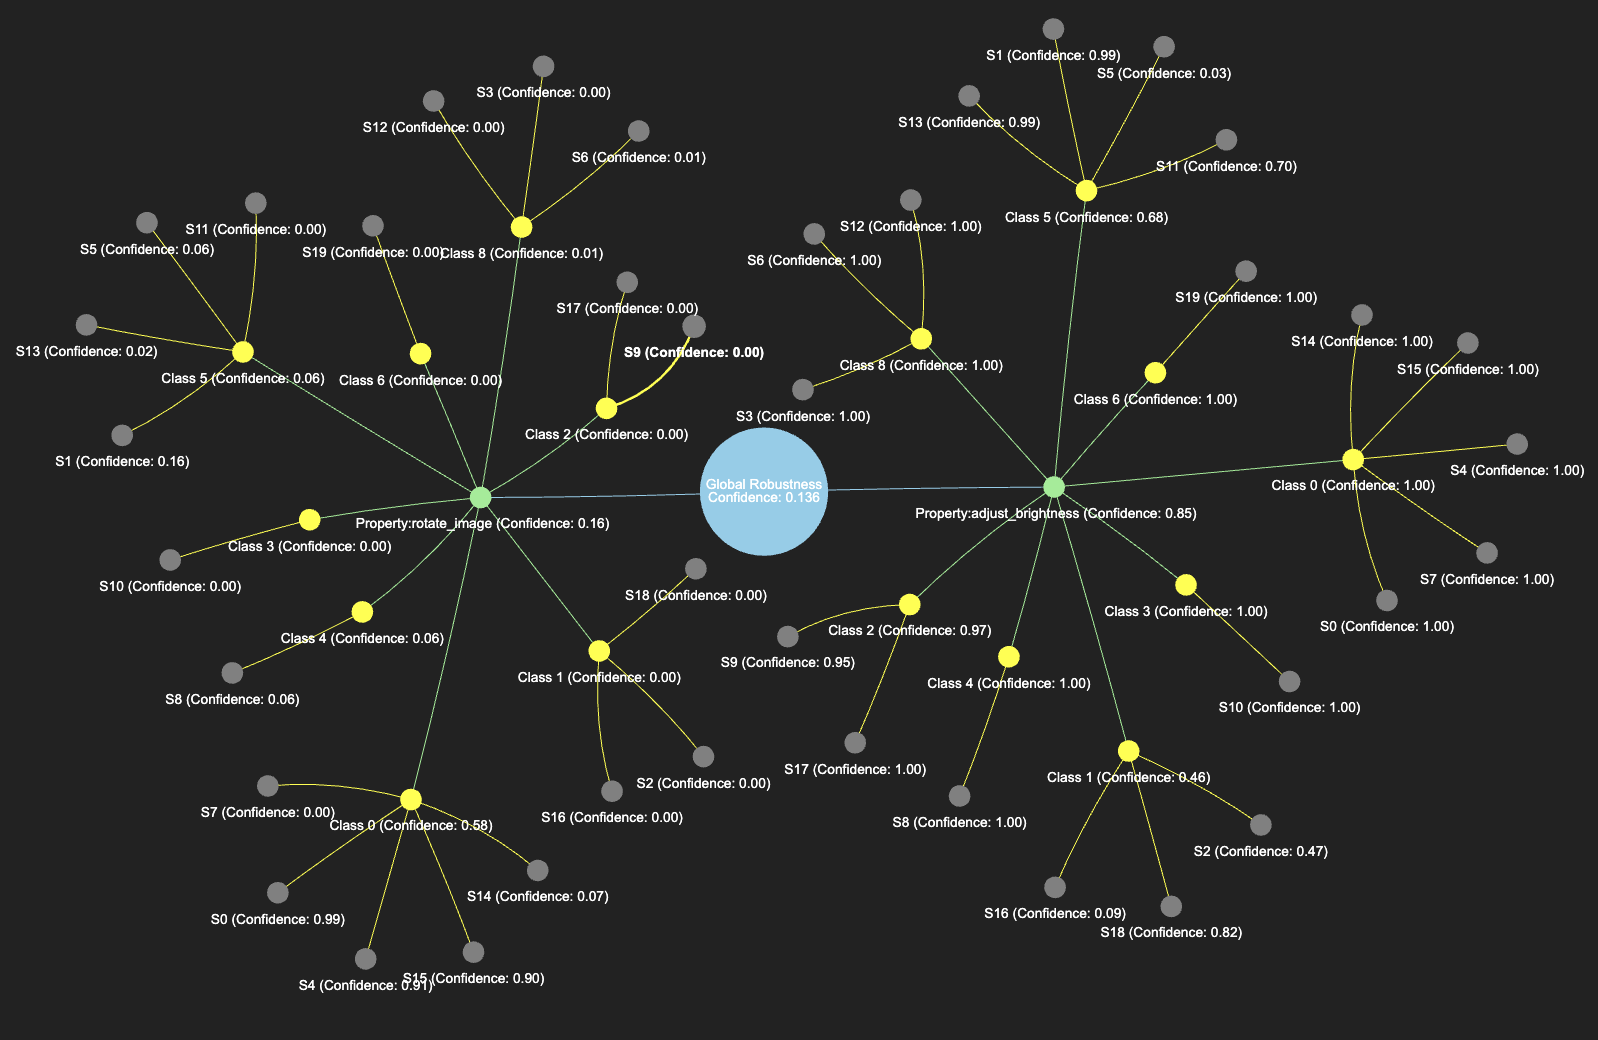
\includegraphics[width=1\textwidth]{Drafts/Experiments/robustness.png}
\caption{Robustness of Model}
\label{}
\end{figure*}






\begin{thebibliography}{01}

\bibitem{Agarwal} Agarwal, Aniya, et al. "Automated test generation to detect individual discrimination in AI models." arXiv preprint arXiv:1809.03260 (2018).

\bibitem{Youcheng} Sun, Youcheng, et al. "Concolic testing for deep neural networks." Proceedings of the 33rd ACM/IEEE International Conference on Automated Software Engineering. 2018.

\bibitem{Kexin} Pei, Kexin, et al. "DeepXplore." Communications of the ACM 62.11 (2019): 137-145.

\bibitem{Yuchi} Tian, Yuchi, et al. "Deeptest: Automated testing of deep-neural-network-driven autonomous cars." Proceedings of the 40th international conference on software engineering. 2018.

\bibitem{Sun} Sun, Youcheng, et al. "Testing deep neural networks." arXiv preprint arXiv:1803.04792 (2018).

\bibitem{Ma} Ma, Lei, et al. "Deepgauge: Multi-granularity testing criteria for deep learning systems." Proceedings of the 33rd ACM/IEEE international conference on automated software engineering. 2018.

\bibitem{Zhang} Zhang, Mengshi, et al. "DeepRoad: GAN-based metamorphic testing and input validation framework for autonomous driving systems." Proceedings of the 33rd ACM/IEEE International Conference on Automated Software Engineering. 2018.

\bibitem{Xie} Xie, Xiaofei, et al. "Deephunter: Hunting deep neural network defects via coverage-guided fuzzing." arXiv preprint arXiv:1809.01266 (2018).

\bibitem{Gopinath}	Gopinath, Divya, et al. "Symbolic execution for deep neural networks." arXiv preprint arXiv:1807.10439 (2018).


\end{thebibliography}
\end{document}
